\section{関連研究}

\subsection{隠れ状態を用いたホテルレビューのレーティング予測}

藤谷ら\cite{fujitani15}は複数のカテゴリにおけるレーティング予測に対して、
Multi-Instance Multi-Label learning for Relation Extraction (MIML-RE)
\cite{mihai12}モデルを用いた手法を提案している。
その手法では、レビュー内の各文毎に予測した隠れレーティングから
レビュー全体のレーティングを予測する。
図\ref{fig:FujitaniRelationsAmongRatingCategories}のように、
文毎のレーティングからレビュー全体のレーティングを予測する際の
カテゴリ間の繋がりを手動で変化させカテゴリ間の関係性を考慮している。
各文の素性にはBag Of Words (BOW)またはBag Of n-gramsを用いている。
各文毎に隠れレーティングを予測することによって
0.4832の正答率が得られることが示された。
また、カテゴリ間の繋がりによって正答率が変化することも示されている。

\begin{figure}
  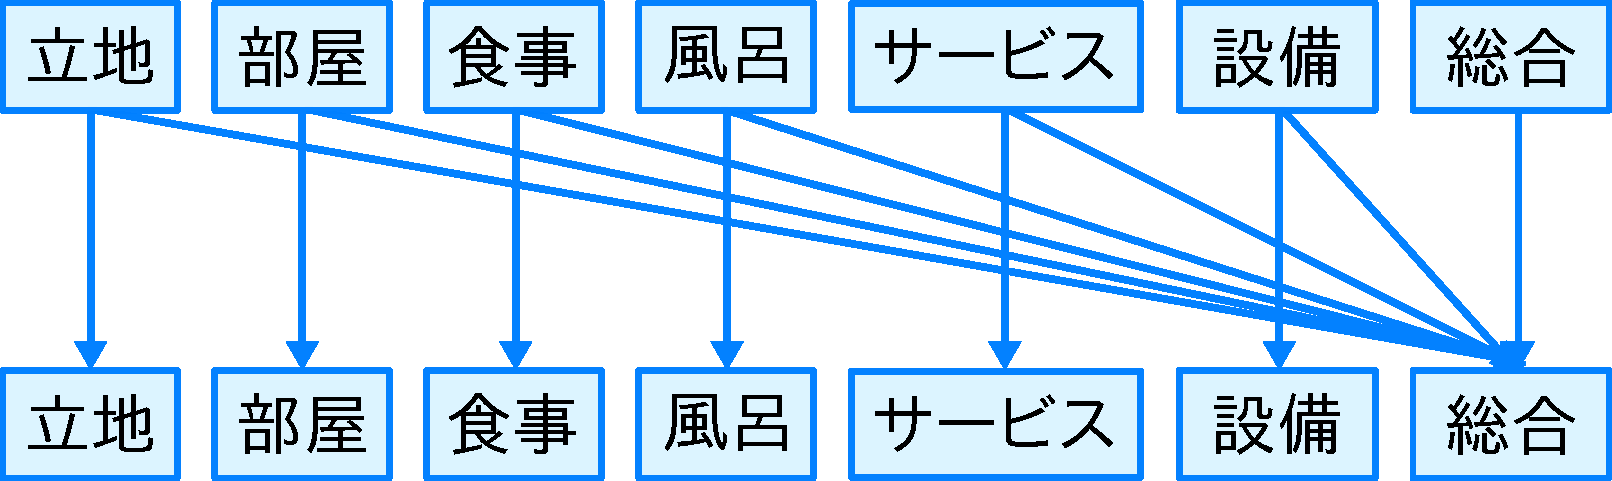
\includegraphics[0.5]
      {fig/fujitani_miml_relations_among_rating_categories.pdf}
  \caption{藤谷ら\cite{fujitani15}のモデルにおけるカテゴリ同士の繋ぎ方の例}
  \label{fig:FujitaniRelationsAmongRatingCategories}
\end{figure}

この手法では、文同士の位置関係を考慮しておらず、
カテゴリ間については考慮しているものの複雑な関係を捉えることができていない。

\subsection{パラグラフベクトル}

パラグラフベクトルは、文や文書といった大きな単位の言語表現の意味表現を
学習する手法である。
これは、Continuous BOW (CBOW)またはSkip-gram\cite{yoshua03}という
単語の意味表現の学習手法を応用した手法である。
ここではCBOWを応用したDistributed Memory model of Paragraph Vectors (PV-DM)
について説明する。
PV-DMはBOWと異なり、単語の並び順を考慮した文や文書の分散表現を
生成することができる。

\begin{figure}
  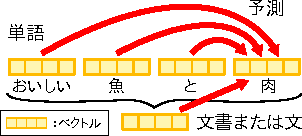
\includegraphics[0.5]{fig/paragraph_vector_v2.pdf}
  \caption{パラグラフベクトルの学習の概略}
  \label{fig:ParagraphVector}
\end{figure}

以下に具体的なアルゴリズムを示す。
ここでは文書の意味表現を学習する場合について考える。
学習の概略を図\ref{fig:ParagraphVector}に示す。
まず、意味表現を学習する対象となる文書に含まれる単語を
初めから一つずつ読んでいく。
その際、現在の単語及びその周辺の単語、現在の文書について、
式\ref{eq:ParagraphVector}に示す目的関数$L$を最大化するように
各パラメータの学習を行う。
\begin{gather}
  L = \frac{1}{T} \sum^{T}_{t = k} \log p(w_t | w_{t-k}, ..., w_{t-1}),
    \label{eq:ParagraphVector} \\
  p(w_t | w_{t-k}, ..., w_{t-1}) = \frac{e^{y_{w_t}}}{\sum_i e^{y_i}},
    \nonumber \\
  y = b + Uh(w_{t-k}, ..., w_{t-1}, d; W, D) \nonumber
\end{gather}
ここで、$d$は文書、$w_i$は単語、$W$は全ての単語の分散表現を表す行列、
$D$は全ての文書の分散表現を表す行列である。
$k$はウィンドウサイズ、$T$は現在の文書に含まれる単語数である。
ある単語の周辺を表す区間をウィンドウという。
$p$はsoftmax関数により正規化された、文脈から現在の単語が導かれることの
尤度である。
$p$を構成する$y$は現在の単語とウィンドウ内の単語及び現在の文書から導出される。
$h(w_{t-k}, ..., w_{t-1}, d; W, D)$は引数となるベクトルを平均したベクトル
または結合したベクトルを返す関数である。

PV-DMによって得られたパラグラフベクトルはレーティング予測において
BOW等に比べ高い正答率を示すことが示されている。
しかし、文書全体にパラグラフベクトルを用いる場合、文同士の位置関係が
予測時に考慮できない。


\subsection{ニューラルネットワークを用いた評判分析}

ニューラルネットワークを用いた評判分析の手法が、Nalら\cite{nal14}、
Rieら\cite{rie14}、Duyuら\cite{duyu15}等によって提案されている。
これらの方法に共通するのは、単語の意味表現から畳み込みニューラルネットワークと
全結合ニューラルネットワークを用いて分類を行うことである。
まず、単語の意味表現から畳み込みニューラルネットワークを
用いて単語同士の関係を捉えた特徴量を抽出する。
その後、そこから得られた文書全体の特徴量を
全結合ニューラルネットワークの入力とし多値または二値分類を行う。
また、Duyuら\cite{duyu15}とNalら\cite{nal14}の手法は
ニューラルネットワークのモデルの中にパラメータとして
単語の意味表現を取り込んでいる。
これにより、特定の分類問題に対してそれらを最適化することができる。

これらの手法は1つのカテゴリにおける多値または二値分類を対象としている。
よって、多カテゴリのレーティング予測において、これらの手法をカテゴリ毎に
適用しただけではカテゴリ間の関係を考慮することができない。
